\documentclass[13]{article}
\newtheorem{exer}{Question}
\usepackage[margin=0.5in]{geometry}
\newtheorem{sln}{Solution}
\usepackage{graphicx}
\newtheorem{note}{Note}
\begin{document}
\section{Lecture 4}
\begin{exer}
What are Mechanical properties of a material reflect ?
\end{exer}

It reflects its response or deformation due to a certain load or force.
\begin{exer}
What factor to be considered in measuring mechanical properties ?
\end{exer}
Factors to be considered include the nature of the applied load and its
duration, as well as the environmental conditions. It is possible for the
load to be tensile, compressive, or shear, and its magnitude may be constant
with time, or it may fluctuate continuously.  Application time may be only a
fraction of a second, or it may extend over a period of many years. Service
temperature and humidity may also be important factors.
\begin{exer}
The most common mechanical test  ?
\end{exer}
The tension test, where a specimen is put under pure axially oriented stress (axial tension). The machine simply keeps increasing the load while measuring the load vs elongation. 
\begin{exer}
How to normalize the tension test regardless of the dimensions of the specimen and load ?
\end{exer}
We divide the load by the \textbf{initial area}  to get the stress
\[
\sigma = \frac{L}{A_0} 
.\] 
and we divide the elongation by the \textbf{initial length }to have the strain. 
\[
\epsilon = \frac{\Delta L}{L} 
.\] 
So instead of the force-elongation curve we get what is called the stress-strain curve.
\\
\begin{center}
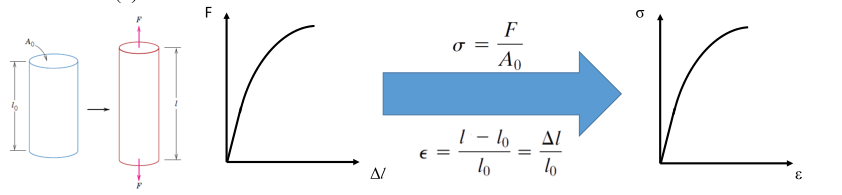
\includegraphics[scale=0.5]{figures/1.png}
\end{center}
\begin{exer}
What do we get from the stress-strain curve ?
\end{exer}
We know the mechanical properties of the material such as: Modulus of Elasticity, Ductility, Resilience, Toughness, UTS, Yield Stress, Allowable stress. (stress or strength)
\begin{exer}
Describe the elastic behaviour ?
\end{exer}
The elastic region or range, is when the tension is at relatively low levels where no bonds are broken, so the material returns to its original shape when The load is removed. Note that the elastic deformation presists only to strains of about 0.005 or (0.5\%).
\begin{exer}
	Where can we find the Yield Stress(Strength) of a material ?
\end{exer}
At the end of the elastic(linear) region.
\begin{exer}
What is young's modulus ? And how do we get it ?
\end{exer}
Young's modulus or the modulus of elasticity (E) is a measure of the material's stiffness. The greater the stiffer the material. \\
We calculate it using the stress-strain graph's elastic region as it is the slope of the linear region. 
\begin{center}
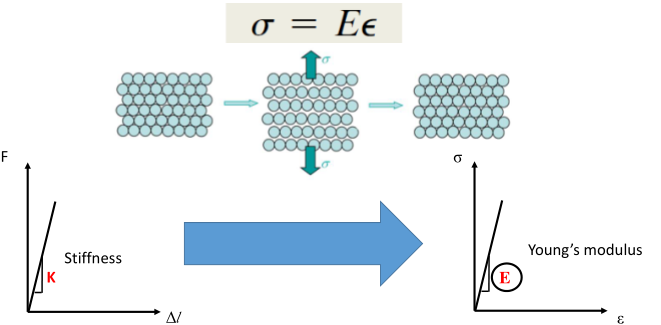
\includegraphics[scale=0.5]{figures/2.png}
\end{center}
\begin{exer}
What are the most stiff elements/materials ?
\end{exer}
Ceramics. They have the highest E.
\begin{exer}
What it the plastic behaviour of a material ?
\end{exer}
After the 0.005 strain (yield strain)  we get to the plastic region, where if the material is deformed in this region it won't get back to its original state or shape. Non-recoverable. In this region there is a slip that happens in the atoms planes.
\begin{center}
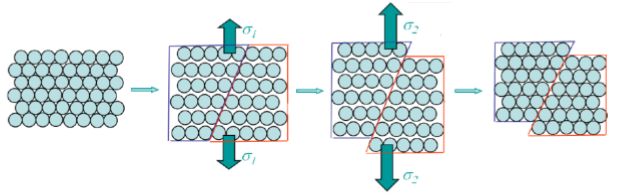
\includegraphics[scale=0.5]{figures/3.png}
\end{center}
\begin{exer}
When does the plastic deformation occur?
\end{exer}
Exactly after the yield stress. $\sigma_y$. At a point P which is called the proportionality limit.
\begin{exer}
	How to find the point P or the yield stress$\sigma_y$ ?
\end{exer}
We go 0.002 (0.2\%) offset, 0.002 of the total deformation (x-axis) and then make a straight line parallel to the elastic region's line. The point we hit is called the P.
\begin{center}
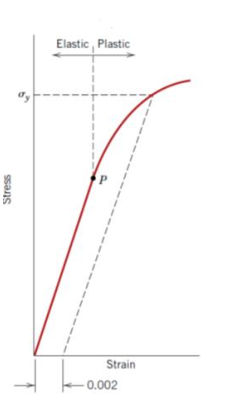
\includegraphics[scale=0.5]{figures/4.png}
\end{center}
\begin{exer}
What is the UTS?
\end{exer}
The ultimate tensile strength, is the stress at the maximum point on the engineering stress-strain curve. After which Necking happens and then the stress decreases as the force decreases and the original area is constant. 
\begin{exer}
What to choose when designing a material to be your safety guideline ?
\end{exer}
We choose the yield strength instead of the ETs and of course divide it by the safety factor in order to get the allowable stress.
\[
	\sigma_{all} = \frac{\sigma_y}{FS} 
.\] 
\begin{exer}
What is Ductility and Brittles ?
\end{exer}
it is a measure of the degree of plastic deformation that has been sustained at fracture . The material that experiences significant plastic deformation until fracture is said to be \textbf{ductile} . (long plastic deformation region).
While the material that exhibits only less than 5\% or no plastic deformation is said to be \textbf{brittle. } 
\begin{exer}
How to calculate Ductility ?
\end{exer}
Well, it is a percent. Percent elongation or percent reduction in area.
\begin{center}
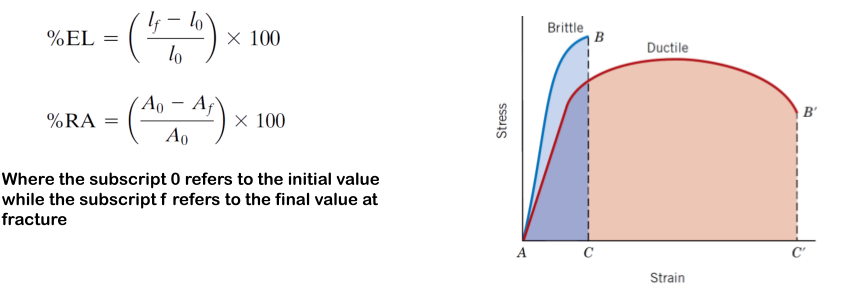
\includegraphics[scale=0.5]{figures/5.png}
\end{center}
\begin{exer}
What is Resilience ?
\end{exer}
it is the capacity of the material to absorb energy while being deformed elastically. And upon unloading this energy is released. It represents the energy per unit volume (Makes sense).   
\begin{exer}
How to measure Resilience ?
\end{exer}
Using the modulus of resilience $U_r$
\[
	U_r = \frac{1}{2} \sigma_y \epsilon_y = \frac{1}{2} \sigma_y (\frac{\sigma_y}{E}) = \frac{\sigma_y^2}{2E} J/m^3 
.\]
\textbf{It is like Spring Energy. The area under the Elastic region Curve
} 
\begin{center}
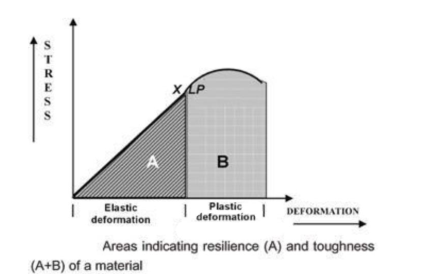
\includegraphics[scale=0.5]{figures/6.png}
\end{center}
\begin{exer}
What is toughness ?
\end{exer}
is the ability of the material to absorb energy and plastically deform before fracturing. Like resilience. 
\begin{exer}
What is the effect of temperature on mechanical properties ?
\end{exer}
We notice from the following graphs that decreasing the temperature decreases the ductility and hence decreases the toughness, but increases the strength of the material.
\begin{center}
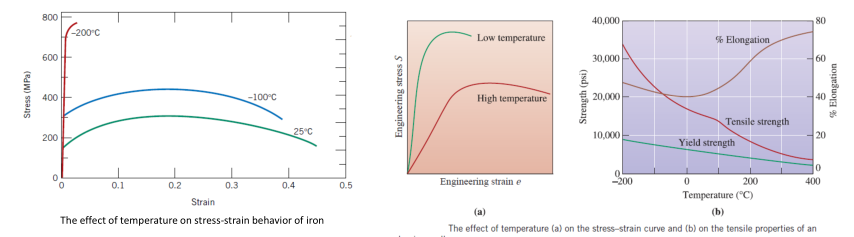
\includegraphics[scale=0.5]{figures/7.png}
\end{center}
\begin{exer}
What is the True stress-strain curve ?
\end{exer}
Instead of the engineering stress-strain curve we have what is called the true stress-strain curve, in which the stress is computed by dividing the current force with the instant's cross sectional area not the original area.
\[
\sigma = \frac{F}{A_i}
.\] 
\begin{exer}
Compare the engineering VS the true stress-strain curve ?
\end{exer}
in the engineering one, after the M point (at which UTS exists), the metal becomes weaker. But this is not true, in face it is increasing in strength. The cross section is decreasing so the stress becomes higher.\\
\begin{exer}
But why does the curve go lower in the engineering one? 
\end{exer}
It is part of the experiment, we choose a certain strain rate to pull the specimen with, So the force needed to pull the specimen decreases with time as the area becomes smaller significantly when necking occurs. The machine decreases the force in order to have the same strain rate.
\begin{exer}
How to calculate the true stress in the curve ?
\end{exer}
\[
\sigma_T = \frac{F}{A_i} 
.\] 
\begin{exer}
How to calculate the true strain ?
\end{exer}
\[
	Elongation = \epsilon_T = \Sigma d\epsilon = \Sigma \frac{dl}{l}=\int \limits_{l_0}^{l} \frac{dl}{l} = ln(l)-ln(l_0) = ln( \frac{l}{l_0})  
.\] 
\begin{exer}
The relationship between the true and engineering stress-strain curves ?
\end{exer}
We can assume that the volume of the specimen is the same (constant) as it deforms \textbf{(but this is before the necking)}  so:
\[
A_0l_0 = Al
.\] 
and Hence:
\[
\sigma_T = \frac{F}{A} = \frac{Fl}{A_0l_0} = \frac{\sigma l}{l_0}
.\] 
\[
l = l_0+\Delta l \\ 
.\] 
\[
\sigma_T = \sigma (1+\frac{\Delta l}{l}) = \sigma (1+ \epsilon)
.\]
and Again
\[
	\epsilon_T = ln(1+ \epsilon)
.\] 
\begin{center}
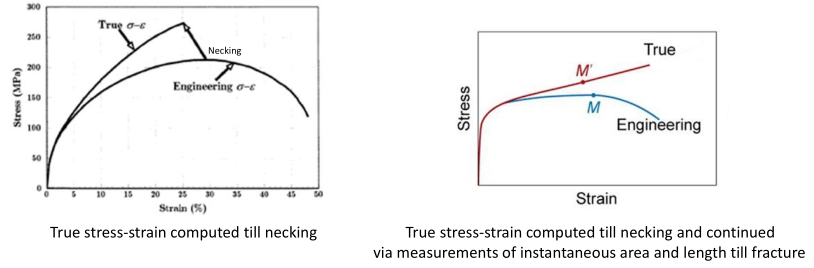
\includegraphics[scale=0.5]{figures/8.png}
\end{center}
\begin{exer}
Define true strain
\end{exer}
The instantaneous elongation per unit length of the specimen.
\begin{exer}
Compare true and engineering stresses and strains.
\end{exer}
The true stress is higher than the Engg. stress, while the true strain is smaller than the Engg. Strain.
\begin{exer}
The relationship between true stress and strain?
\end{exer}
\[
\sigma_T = K \epsilon_T^n
.\] 
This is called the flow stress, K and n are constants and they vary from one metal or alloy to the other. N is called the strain hardening exponent, it is less than 1. 
\section{Lecture 5}
\begin{exer}
	What other tests can we use to find mechanical properties ?
\end{exer}
Three point bend test - impact test - hardness test
\end{document}


